\section{Анализ литературных источников, прототипов и формирование требований к проектируемому программному средству}
\label{sec:analysis}

Конечный успех программного проекта во многом определяется до начала конструирования: на этапе подготовки, которая проводится с учетом всех особенностей проекта.

Первое предварительное условие, которое нужно выполнить перед конструированием, -- ясное формулирование проблемы, которую система должна решать. Общая цель подготовки — снижение риска: адекватное планирование позволяет исключить главные аспекты риска на самых ранних стадиях работы, чтобы основную часть проекта можно было выполнить максимально эффективно. 

Главный факторы риска в создании ПО — неудачная выработка требований. Требования подробно описывают, что должна делать программная система. Внимание к требованиям помогает свести к минимуму изменения системы после начала разработки \cite{code_complete}.

Перед формулированием требований необходимо изучить ряд вопросов, которые напрямую влияют на все дальнейшие этапы разработки. В частности, необходимо рассмотреть вопросы выбора платформ, архитектуры. По результатам анализа можно будет составить техническое задание к проектируемому программному средству, которое станет основой для составления функциональных требований.

\subsection{Аналитический обзор литературных источников}
\label{sec:analysis:literature}

Далее приводится анализ сведений, которые влияют на формулирование требований, выбор архитектуры и дальнейшее проектирование и разработку программного средства.

\subsubsection{} Кроссплатформенность приложений
\label{sec:analysis:literature:crossplatform}

Как несколько десятилетий назад, так и в настоящее время выбор платформы является серьезным ограничением для всех последующих этапов разработки. Однако уже начали появляться технологии, которые позволяют использовать однажды написанный код на многих платформах. Сегодня все больше приложений создается сразу для нескольких платформ, а приложения, созданные изначально для одной платформы, активно адаптируются под другие \cite{habr_crossplatform}. Разработчик, изучающий какую-либо из таких технологий, получает конкурентное преимущество, поскольку за счет расширения количества платформ расширяется круг задач, над которыми он может работать. Поэтому кроссплатформенность -- реальная или потенциальная -- является одним из факторов, который необходимо учитывать при выборе технологий реализации проекта.

\subsubsection{} Обзор целевых платформ
\label{sec:analysis:literature:platforms}

Несмотря на планируемое использование кроссплатформенных технологий, поддержка всех платформ может затребовать значительно больших сред\-ств и времени, чем есть в наличии для выполнения дипломного проектирования. Поэтому, необходимо осуществить выбор одной основной платформы с расчетом на продолжение разработки и реализацию проекта для других платформ. Рассмотрим достоинства и недостатки основных.

\emph{Настольное приложение} -- программное средство, которое запускается локально на компьютере пользователя. При его создании появляется возможность использования всех преимуществ аппаратного обеспечения, которым оснащен компьютер, например: прямой доступ к видеокарте, внешним устройствам. Кроме того, появляется возможность взаимодействия с другими установленными приложениями.

Тем не менее у настольных приложений есть и ряд недостатков. Когда пользователь работает удаленно, возникают проблемы, связанные с сетью, соединениями, сетевыми экранами. Один из самых больших недостатков заключается в огромной сложности развертывания приложения на десятки или сотни машин, их конфигурирования, периодического обновления \cite{msdn_desktop_vs_web}.

\emph{Веб-приложения}, в отличие от настольных, работают на удаленном аппаратном обеспечении и поставляются пользователю через браузер \cite{web_based_vs_desktop}. При их использовании разработчик избавляется от необходимости поддерживать установку большого числа зависимостей, он всегда может быть уверен, что все пользователи используют самую последнюю версию приложения. Вычислительные операции могут производиться на мощном сервере, а результаты вычислений поставляться пользователю -- так называемая концепция <<тонкого клиента>> \cite{desktop_vs_web_deeper_look}.

Несмотря на то, что ресурсоемкие вычисления производятся на сервере, задержки при передаче, особенно при нестабильном соединении, сама потребность в постоянном интернет соединении могут значительно снизить удобство пользования приложением. Кроме того, размер загружаемого при каждом запуске кода и ресурсов может значительно увеличить траты пользователя, особенно если он использует дорогое мобильное подключение к интернету.

Для \emph{мобильных приложений} актуальны ограничения платформ, на которых они запускаются, такие как меньшие размеры экранов, более медленные процессоры, ограниченное энергопотребление. Несмотря на это, мобильные устройства часто находятся рядом с пользователями, появляется возможность использования мгновенных оповещений \cite{desktop_mobile_differences}. Вместе с этим, большинство смартфонов оснащено модулями, такими как GPS, камера, NFC, что пре\-дос\-тав\-ля\-ет разработчику новые возможности по их использованию.

На основании рассмотренных характеристик различных платформ можно осуществить выбор одной из них, которая и станет целевой для разработки.

\subsubsection{} Обзор архитектурных стилей
\label{sec:analysis:literature:architecture}

Далее необходимо рассмотреть применяющиеся на практике архитектурные стили, провести их анализ и по результатам осуществить выбор архитектуры, которая затем будет применяться при проектировании программного средства.

Под разработкой \emph{архитектуры} понимают специфицирование структуры всей системы: глобальную организацию и структуру управления, протоколы коммуникации, синхронизации и доступа к данным, распределение функциональности между компонентами системы, физическое размещение, состав системы, масштабируемость и производительность \cite{introduction_to_architecture}. Набор принципов, используемых в архитектуре, формирует \emph{архитектурный стиль}. Применение архитектурных стилей упрощают решение целого класса абстрактных проблем \cite{architecture_volosevich}.

При проектировании архитектуры программной системы почти никогда не ограничиваются единственным архитектурным стилем, поскольку они могут предлагать решение каких-либо проблем в различных областях. В таблице~\ref{table:analysis:architectures:categorization} приведен вариант категоризации архитектурных стилей \cite{application_architecture_guide}.

\begin{table}[ht]
\caption{Категоризация архитектурных стилей}
\label{table:analysis:architectures:categorization}
\centering
  \begin{tabular}{|>{\raggedright}m{0.27\textwidth} 
                  |>{\raggedright\arraybackslash}m{0.675\textwidth}|}
  \hline Категория & Архитектурный стиль \\
  \hline Связь & SOA (Service-oriented architecture -- архитектура, ориентированная на сервисы), Шина сообщений \\
  \hline Развертывание & Клиент-серверный, трехуровневый, N-уровневый \\
  \hline Предметная область & DDD (Domain-driven design -- проблемно-ориентированное проектирование) \\
  \hline Структура & Компонентный, объектно-ориентированный, многоуровневый\\
  \hline
  \end{tabular}
\end{table}

\emph{Сервис-ориентированная архитектура} позволяет приложениям предоставлять некоторую функциональность с помощью набора слабосвязанных автономных сервисов; связь между сервисами обеспечивается с помощью заранее определенных контрактов. Данный стиль предоставляет следующие преимущества \cite{application_architecture_guide}:

\begin{itemize}
	\item повторное использование сервисов снижает стоимость разработки;
	\item автономность и использование формальных контрактов способствует слабой связанности и повышает уровень абстракции;
	\item сервисы могут использовать возможность автоматического обнаружения и определения интерфейса;
	\item сервисы и использующие их приложения могут быть развернуты на различных платформах.
\end{itemize}

Архитектура \emph{шины сообщений} описывает принципы построения систем, которые используют обмен сообщениями как способ связи. Наиболее часто при реализации данной архитектуры используется модель маршрутизатора сообщений или шаблон издатель-подписчик. Главные преимущества использования данного архитектурного стиля \cite{application_architecture_guide}:

\begin{itemize}
	\item расширяемость, которая заключается в возможности добавлять и удалять приложения без влияния на другие;
	\item снижается сложность приложений, так как единственный интерфейс, который они должны поддерживать -- интерфейс общей шины;
	\item гибкость, которая заключается в возможности подстраиваться под биз\-нес-требования или желания пользователей через изменения конфигурации или параметров маршрутизации сообщений;
	\item слабая связанность, поскольку единственное, чем связаны приложения -- интерфейс общей шины;
	\item масштабируемость, которая заключается в возможности в случае необходимости присоединения к шине нескольких экземпляров одного и того же приложения.
\end{itemize}

\emph{Клиент-серверная архитектура} описывает распределенную систему, которая включает независимые системы сервера, клиента и соединяющую их сеть. Иногда данную архитектуру называют двухзвенной. Из преимуществ выделяют следующие \cite{architecture_volosevich}:

\begin{itemize}
	\item безопасность: все данные хранятся на сервере, обеспечивающем больший уровень безопасности, чем отдельные клиенты;
	\item централизованный доступ к данным, который предоставляет возможность более легкого управления, чем в других архитектурах;
	\item устойчивость и легкость поддержки: роль сервера могут выполнять несколько физических компьютеров, объединённых в сеть; благодаря этому клиент не замечает сбоев или замены отдельного серверного компьютера.
\end{itemize}

\emph{Многоуровневая архитектурный стиль} заключается в группировании\linebreakсхожей функциональности приложения по уровням, которые выстроены в вертикальную структуру. Уровни связаны слабо, связь между ними осуществляется по явно установленным протоколам. Строгий вариант архитектуры предполагает, что компоненты какого-либо уровня могут взаимодействовать только с компонентами одного нижележащего уровня; ослабленный вариант разрешает взаимодействие с компонентами любого из нижележащих уровней. Использование данного архитектурного стиля предлагает следующие преимущества \cite{application_architecture_guide}:

\begin{itemize}
	\item есть возможность осуществлять изменения на уровне абстракций;
	\item изолированность: изменения на каких-либо уровнях не влияют на другие, что снижает риск и минимизирует воздействие на всю систему;
	\item разделение функциональности помогает управлять зависимостями, что приводит к большей управляемости всего кода;
	\item независимые уровни предоставляют возможность повторного использования компонентов;
	\item строго-определенные интерфейсы способствуют повышению тестируемости компонентов.
\end{itemize}

\emph{Многозвенная архитектура} предлагает схожее с многоуровневой архитектурой разбиение функциональности, отличие же заключается в предлагаемом размещении звеньев на физически обособленной машине \cite{architecture_volosevich}. Предлагается использовать данный стиль в случаях, когда компоненты одного звена могут проводить дорогие в ресурсном отношении вычисления, так что это может сказаться на других уровнях, или когда некоторую чувствительную информацию переносят со звеньев уровня представления на уровень бизнес-логики приложения. Далее приведены главные преимущества использования многозвенной архитектуры:

\begin{itemize}
	\item удобство сопровождения, которое заключается в возможности внесения изменений и обновлений в некоторые компоненты при минимальном влиянии на всё приложение;
	\item масштабируемость, которая возникает из распределенного развертывания;
	\item гибкость, которая появляется благодаря предыдущим двум пунктам;
	\item масштабируемость также приводит к повышению доступности приложения.
\end{itemize}

\emph{Проблемно-ориентированный архитектурный стиль} основывается на\linebreakпредметной области, ее элементах, их поведении и связях между ними. Для применениях данного стиля необходимо иметь хорошее понимание предметной области или людей, которые бы смогли объяснить ее специфику разработчикам. Первое, что нужно сделать при принятии данного стиля -- выработать единый язык, который бы знала вся команда разработчиков, который бы был избавлен от технических жаргонизмов и содержал только термины предметной области -- только так можно избежать проблемы непонимания между участникам \cite{ddd_quickly}. Преимущества, которые может предложить данный стиль:

\begin{itemize}
	\item упрощение коммуникации между участниками процесса разработки благодаря выработке единого языка;
	\item модель предметной области обычно является расширяемой и гибкой при изменениях условий и бизнес-требований;
	\item хорошая тестируемость.
\end{itemize}

\emph{Компонентная архитектура} основывается на декомпозиции системы в отдельные функциональные или логические компоненты, которые раскрывают другим компонентам только заранее определенные интерфейсы \cite{application_architecture_guide}. Преимущества данного подхода:

\begin{itemize}
	\item легкость развертывания, которая заключается в обновлении компонентов без влияния на другие;
	\item использование компонентов сторонних разработчиков позволяет снизить расходы на разработку и поддержку;
	\item поддержка компонентами заранее определенных интерфейсов позволяет упростить разработку;
	\item возможность переиспользования компонентов также оказывает влияние на снижение стоимости.
\end{itemize}

\emph{Объектно-ориентированный архитектурный стиль} выражается в разделении функциональности системы на множество автономных объектов, каждый из которых содержит некоторые данные и набор методов поведения, свойственных объекту. Обычной практикой является определение классов, соответствующих объектам предметной области. Применение данного стиля предоставляет следующие преимущества \cite{application_architecture_guide}:

\begin{itemize}
	\item соотнесение классов программы и объектов реального мира делает программное средство более понятным;
	\item полиморфизм и принцип абстракции предоставляет возможность повторного их использования;
	\item инкапсуляция повышает тестируемость объектов;
	\item улучшение расширяемости, которое возникает благодаря тому, что изменения в представлении данных не оказывают влияния на внешний интерфейс объекта, что не ограничивает его способность взаимодействовать с другими объектами;
	\item высокая сцепленность объектов, которая достигается использованием разных объектов для разного набора действий.
\end{itemize}

Таким образом, применение рассмотренных архитектур на этапе проектирования окажет большое влияние на успешность всего процесса разработки; какие бы стили не были применены, можно быть уверенным в правильности выбора за счет того, что у всех из них есть определенные и зачастую разные преимущества.

\subsubsection{} Проектирование баз данных
\label{sec:analysis:literature:db}

В настоящее время сложно представить сложные приложения, которые бы не использовали специальные средства для хранения информации.

База данных -- представленная в объективной форме совокупность самостоятельных материалов, систематизированных таким образом, чтобы эти материалы могли быть найдены и обработаны с помощью ЭВМ. Модель базы данных -- описание базы данных с помощью  определенного (в т.ч. графического) языка на некотором уровне абстракции.

Основные задачи проектирования баз данных:
\begin{itemize}
	\item Обеспечение хранения в БД всей необходимой информации.
	\item Обеспечение возможности получения данных по всем необходимым запросам.
	\item Сокращение избыточности и дублирования данных.
	\item Обеспечение целостности базы данных.
\end{itemize}

Выделяют следующие уровни моделирования \cite{kulikov_db_workbook}:
\begin{itemize}
	\item инфологический уровень: описание предметной области без привязок к каким-либо средствам реализации: языкам программирования, СУБД, и т.д;
	\item даталогический уровень: модель предметной области в привязке к сре\-д\-с\-т\-вам реализации;
	\item физический уровень: описывает конкретные таблицы, связи, индексы, методы хранения, настройки производительности, безопасности и т.д.
\end{itemize}

При ошибках моделирования могут возникать аномалии операций с БД. Аномалия -- противоречие между моделью предметной области и моделью данных, поддерживаемой средствами конкретной СУБД~\cite{kulikov_db_workbook}.

Выделяют следующие виды аномалий:
\begin{itemize}
	\item Аномалия вставки: при добавлении данных, часть которых у нас отсутствует, мы вынуждены или не выполнять добавление или подставлять пустые или фиктивные данные.
	\item Аномалия обновления – при обновлении данных мы вынуждены обновлять много строк и рискуем часть строк «забыть обновить».
	\item Аномалия удаления – при удалении части данных мы теряем другую часть, которую не надо было удалять.
\end{itemize}

Для устранения аномалий существует процесс нормализации БД.

Нормализация -- группировка и/или распределение атрибутов по отношениям с целью устранения аномалий операций с БД, обеспечения целостности данных и оптимизации модели БД.

Отношение находится в первой нормальной форме, если все его атрибуты являются атомарными. Атрибут считается атомарным, если в предметной области не существует операции, для выполнения которой понадобилось бы извлечь часть атрибута.

Отношение находится во второй нормальной форме, если оно находится в первой нормальной форме, и при этом  любой атрибут, не входящий в состав ПК, функционально полно зависит от ПК.

Отношение находится в третьей нормальной форме, если оно находится во второй нормальной форме, и при этом любой его неключевой атрибут нетранзитивно зависит от первичного ключа~\cite{kulikov_db_workbook}.

Как правило, третья нормальная формы принимается достаточной и, поскольку дальнейшая нормализация может породить избыточность, то она обычно не проводится.


\subsection{Обзор существующих аналогов}
\label{sec:analysis:analogues}

Для решения задач управления временем, задачами и контактами могут использоваться различные средства. Рассмотрим каждую из задач в\linebreakотдельности.
\newline
\subsubsection{} Управление временем и расписаниями
\label{sec:analysis:analogues:schedules}

Для участников учебного процесса управление временем заключается в следовании расписанию, составляемое деканатами или диспетчерской службой университетов. Еще тридцать лет назад расписание представляло собой таблицу на огромном листе бумаги, которую составляли вручную и вывешивали на доске объявлений. Чтобы узнать, какое занятие будет следующим, приходилось или заранее переписывать своё расписание всем студентам, или каждый раз идти к доске объявлений (что имеет свои преимущества, так как тогда есть возможность узнать обо всех изменениях в расписании).

С течением времени от ручного заполнения перешли к составлению электронных таблиц в специальных программных средствах. Тем не менее, облегчено было только составление расписания, а не пользование им: электронные таблицы печатались и по-прежнему вывешивались около деканатов. Потребовалось еще несколько лет и прогресс в развитии информационных технологий, чтобы студенты и преподаватели получили возможность получения расписания через сеть интернет без необходимости посещения университета.

В настоящее время на постсоветском пространстве существует огромное число высших учебных заведений. Некоторое время назад процессы, происходящие в таких учреждениях не были оцифрованы и автоматизированы вовсе. Лишь недавно начали появляться информационные системы, решающие те или иные задачи. Однако, каждый ВУЗ занимается этой проблемой самостоятельно и решает ее, насколько хватает квалифицированных специалистов, ресурсов и, самое главное, желания внедрять что-то инновационное со стороны руководства и участников учебного процесса этих ВУЗов.

Универсальной шкалы, позволяющей оценить удобство следования по всем деятельностям учебного процесса в разных ВУЗах, нет. Однако, можно попытаться это оценить по некоторым вторичным признакам, таким как, например, соответствие сайта ВУЗа современным представлениям об удобстве пользования (можно легко отличить сайты, сделанные за последние несколько лет, от сайтов, сделанных более десяти лет назад: со временем меняются и представления об удобстве пользования, и технологии, позволяющие его достичь), отзывах тех людей, которые участвуют в процессе обучения (то есть студентов, преподавателей) и некоторым другим. Рассмотрим возможности, предоставляемые информационными системами различных белорусских ВУЗов по состоянию на апрель 2017 года.

Белорусский государственный университет информатики
как ведущий специализированный университет в области информационных технологий на постсоветском пространстве обладает достаточным числом квалифицированных специалистов (поскольку обучает их), чтобы автоматизировать многие части учебного процесса. Для пользования предоставляется система расписания: занятий и экзаменов для студентов и преподавателей, причём предоставляется возможность не только просматривать расписание, находясь на сайте (пример расписания приведен на рисунке \ref{fig:analysis:analogues:bsuir}), но реализован API для получения актуальных данных о преподавателях, группах и расписании для них в формате XML. Помимо этого, наиболее близкий к информационным технологиям факультет компьютерных систем и сетей (КСиС) имеет в своём распоряжении портал факультета, на котором присутствует актуальная информация о событиях, происходящих на факультете, куда выкладываются расписания учебного процесса, списки групп, рейтинговые списки. Однако, по-прежнему существует и ряд проблем. Кроме факультета КСиС, своих порталов не имеет ни один из других факультетов, поэтому вся коммуникация со студентами может происходить только очно, а некоторые неформальные виды коммуникации -- через группы факультетов в социальных сетях. Кафедры не имеют удобной для студентов доски объявлений (строго говоря, такие доски есть, но она находится настолько глубоко внутри сайта университета, что большая часть студентов о ней и не знает). Для того, чтобы внести любое малейшее изменение в расписание, преподавателю нужно обращаться в диспетчерскую службу: нет возможности сделать это автоматически. Но несмотря на все недостатки, БГУИР все равно обгоняет многие ВУЗы по степени информатизации и автоматизации учебного процесса.

\begin{figure}
	\centering
	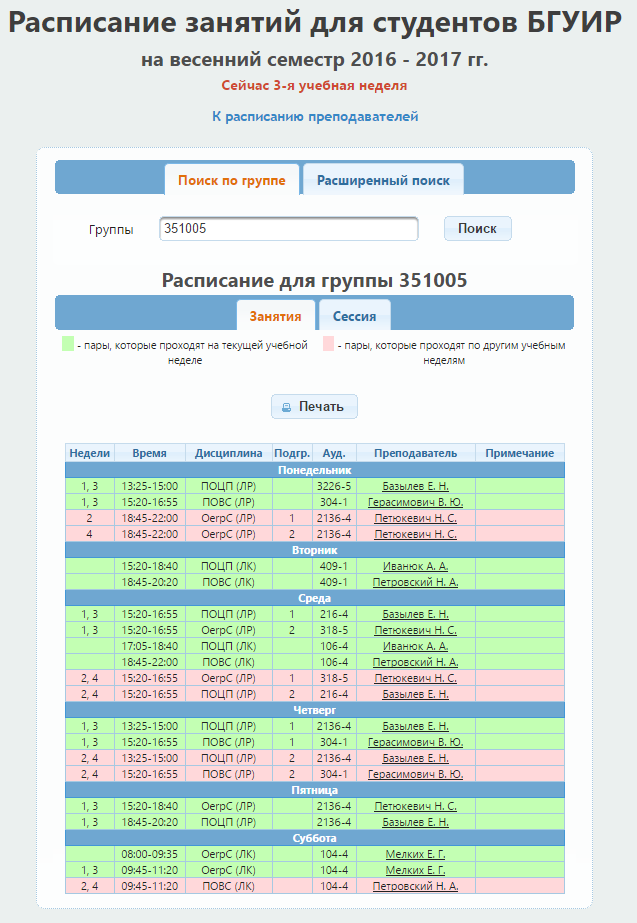
\includegraphics[scale=1]{schedule_bsuir_351005.png} 
	\caption{Пример расписания БГУИР}
	\label{fig:analysis:analogues:bsuir}
\end{figure}

\begin{figure}
	\centering
	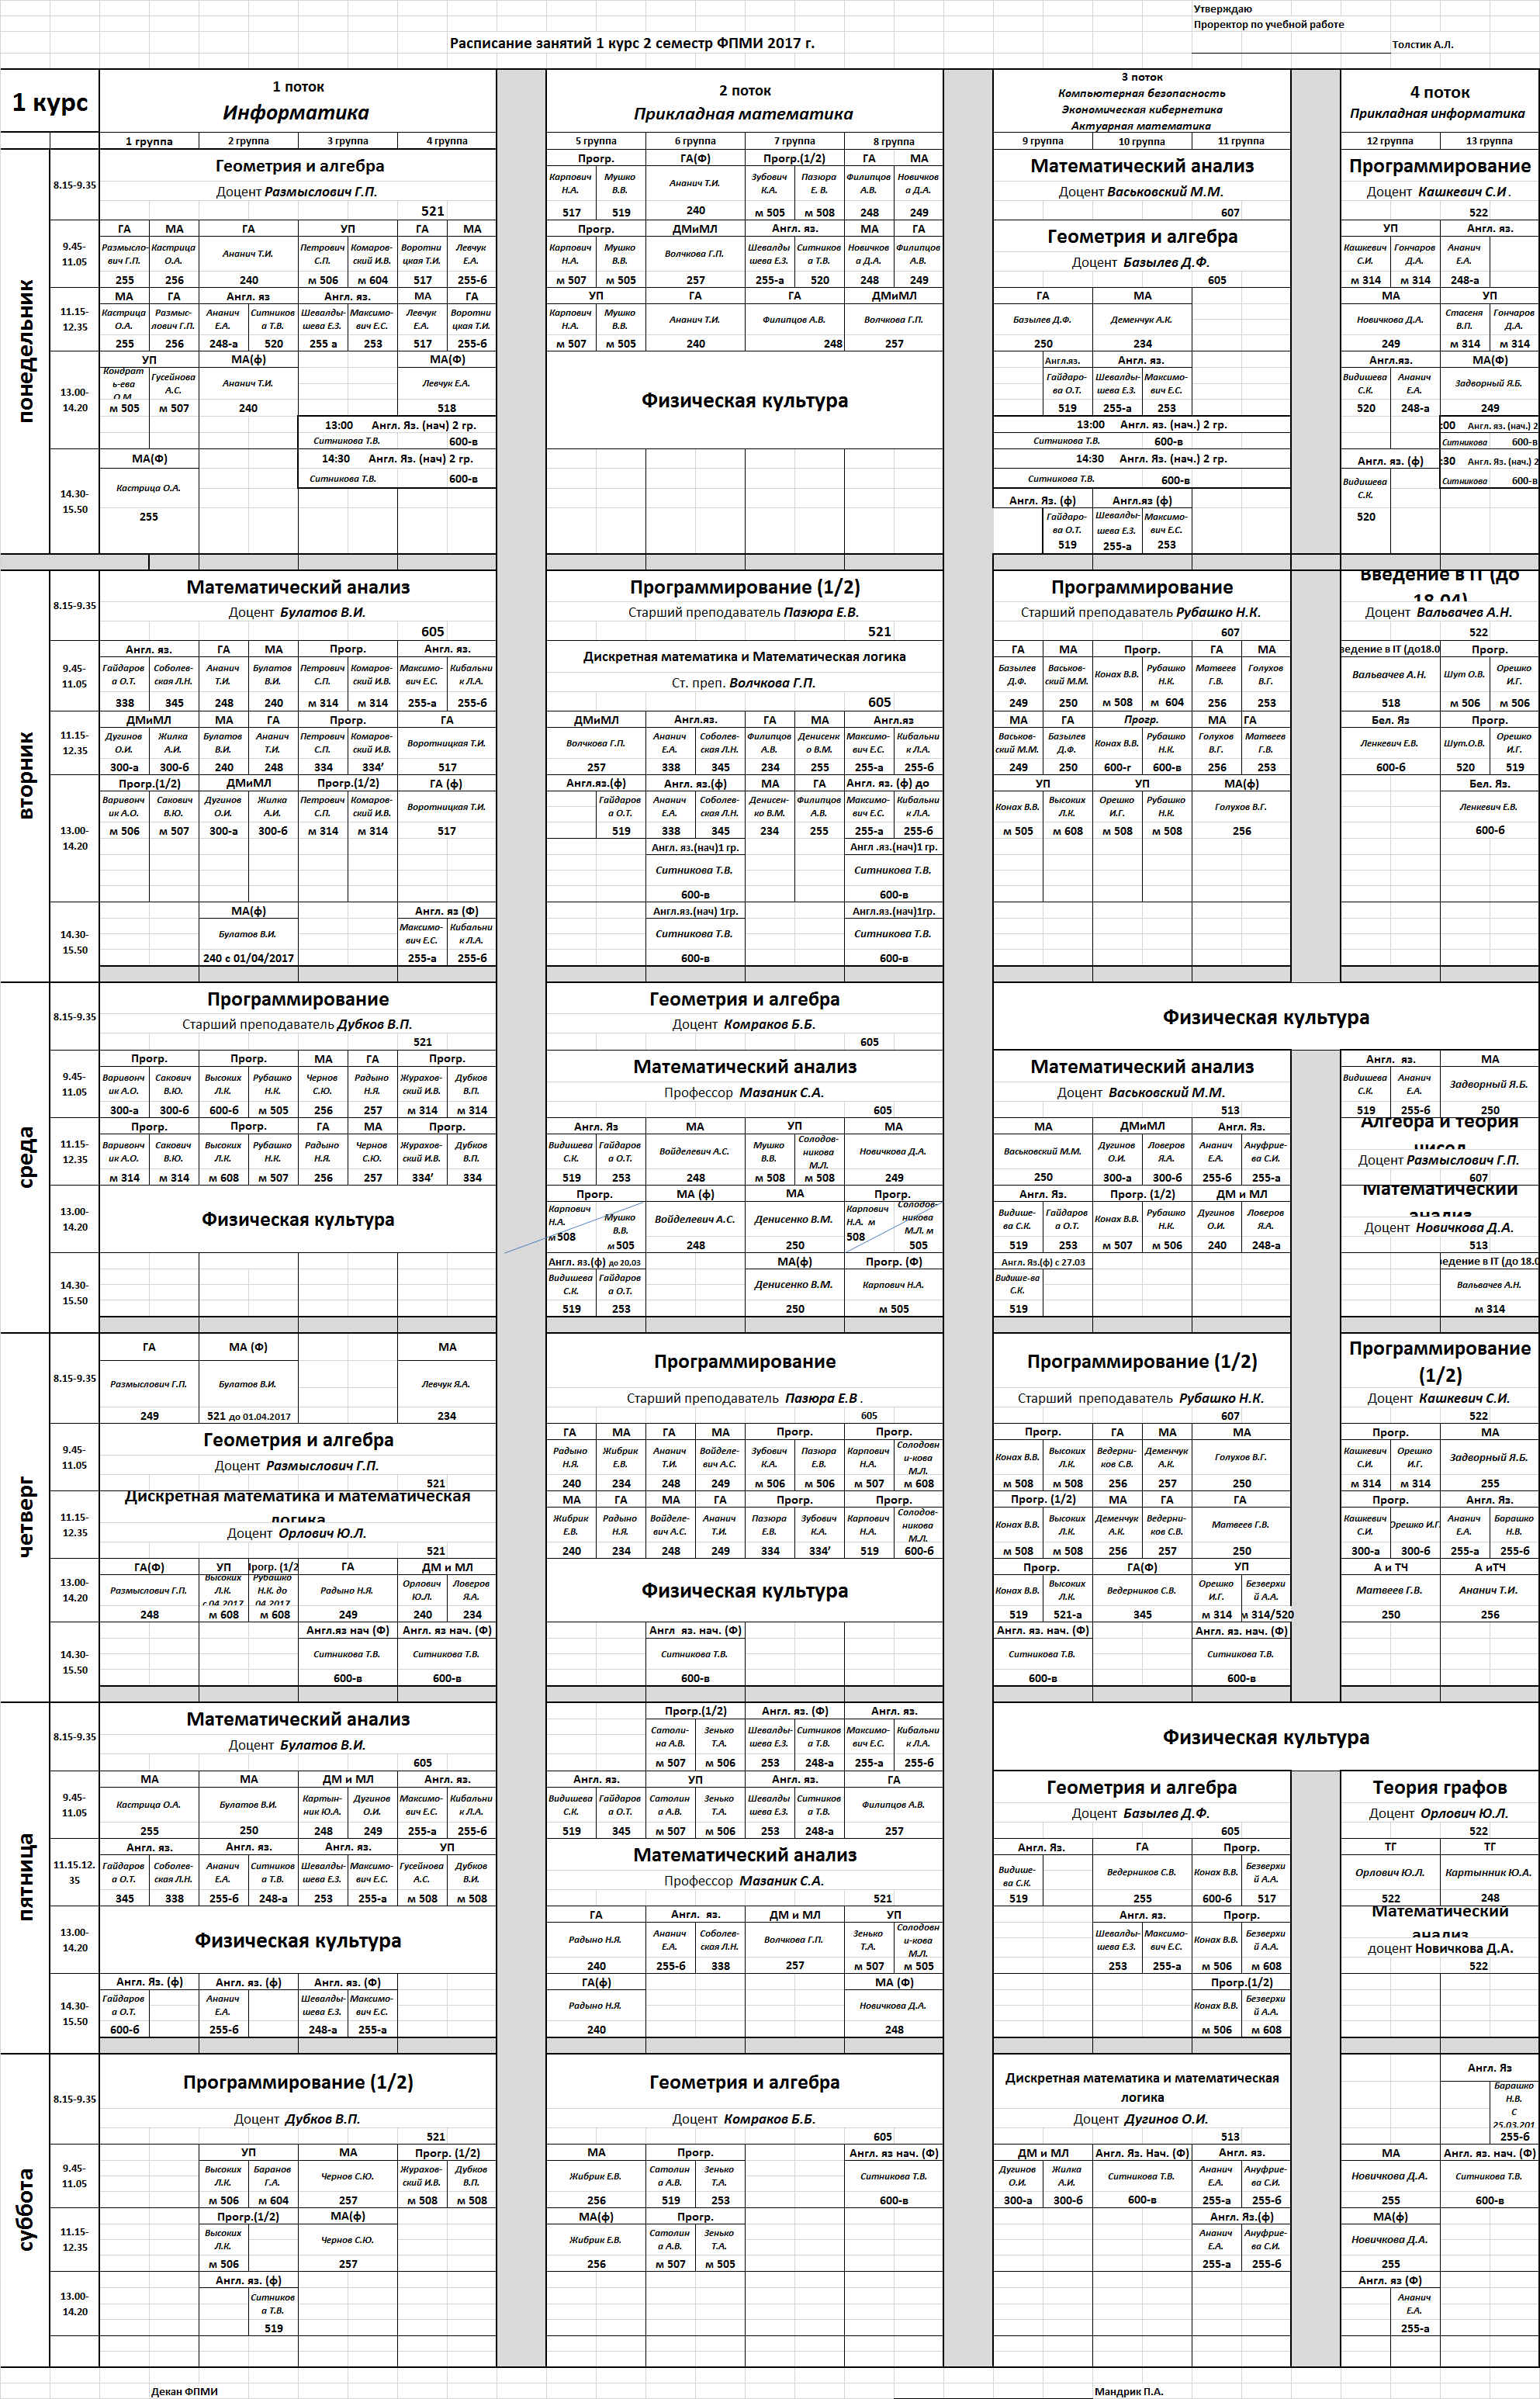
\includegraphics[scale=0.305]{schedule_bsu_fpmi_1kurs.png}
	\caption{Пример расписания ФПМИ БГУ}
	\label{fig:analysis:analogues:bsu_fpmi}
\end{figure}

Сайт ведущего университета страны общего профиля -- Белорусского государственного университета -- был значительно переработан около двух лет назад (то есть около февраля 2015 г.), что привело к значительному повышению удобства пользования и актуальности информации. Еще одним достоинством информационной системы БГУ является то, что для всех факультетов реализованы отдельные порталы. Однако, очень большим недостатком является то, что в этом университете не реализована единая система управления расписанием. Все факультеты решают задачу составления расписания и доставки его студентам и преподавателям по-своему. Есть факультеты, которые предоставляют более-менее удобные таблицы с расписанием (например, на рисунке \ref{fig:analysis:analogues:bsu_fpmi} приведен пример расписания первого курса ФПМИ), есть факультеты, которые предоставляют мобильное приложение с расписанием (но только с расписанием этого факультета), однако, есть факультеты, которые предоставляют расписание в виде неизменяемого и недоступного для автоматизированного разбора документа (например, в формате PDF). Более того, некоторые кафедры вообще не выкладывают своё расписание на сайт факультета, и чтобы студенты и преподаватели могли с ним ознакомиться, им нужно приходить к доске объявлений своей кафедры. В итоге, нет ни программного интерфейса для доступа к расписанию, ни даже унифицированной системы расписания, что значительно затрудняет создание любых приложений для работы с ним. И эту проблему в данном ВУЗе можно решить только одним способом: предложить систему, форматы данных и программные интерфейсы и каким-либо образом убедить их использовать. Но процесс информатизации не стоит на месте, и стоит ожидать, что уже скоро такая унификация произойдёт.

Попытка нивелировать неудобства пользования официальными источниками расписания может состоять в использовании специализированных сер\-висов-календарей. Как и все веб-приложения, они доступны на любом компьютере, подключенном к сети интернет, кроме того, зачастую разработаны официальные приложения для мобильных устройств. Еще одним достоинство является универсальность, заключающаяся в том, что данные сервисы можно использовать не только для управления занятиями университета. Главным же недостатком является необходимость вручную заполнять все расписание (что, однако, даёт возможность самому настроить форму его отображения). Таким образом, на конфигурирование таких приложений может уходить несколько часов пару раз в год. Пример расписания, сформированного с помощью веб-сервиса Google Calendar приведен на рисунке \ref{fig:analysis:analogues:google_calendar}. 

\begin{figure}[!h]
	\centering
	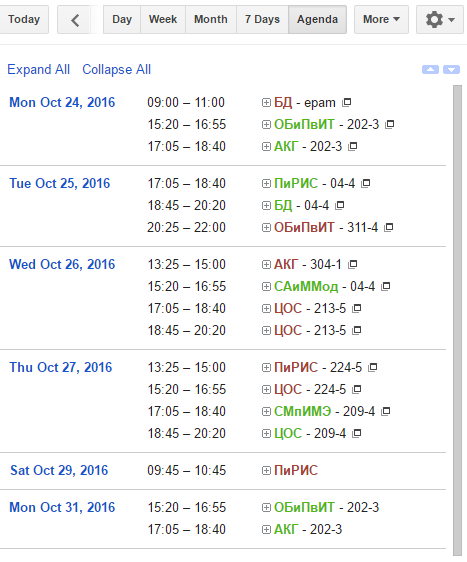
\includegraphics[scale=1]{google_calendar_agenda.png} 
	\caption{Пример расписания, сформированного с помощью сервиса Google Calendar}
	\label{fig:analysis:analogues:google_calendar}
\end{figure}

Анализ существующих информационных систем показывает наличие\linebreakразрозненности, отсутствие единого протокола обмена и хранения данных уче\-б\-но\-го процесса, что подтверждает актуальность разработки программного обе\-с\-пе\-че\-ния, направленного на автоматизацию данной области.

\subsubsection{} Управление задачами
\label{sec:analysis:analogues:tasks}

Управление задачами заключается в их учете и ранжированию по приоритету. Для этого могут использоваться различные записные книги и календари.

Самым первым средством стали обычные бумажные записные книги. И по сей день есть большое число их сторонников, для которых оказывается намного более удобным записать какие-то идеи на бумаге, чем в приложении на мобильном устройстве или компьютере \cite{paper_notebooks_power}. Из преимуществ выделяют следующие:

\begin{itemize}
	\item доступность, которая заключается в привычке постоянно держать бло\-к\-нот около себя;
	\item надежность, которая обусловлена независимостью от сети интернет и источников питания;
	\item визуализация и фиксация мыслей на бумаге часто помогает лучше обдумать задачу;
	\item универсальность: блокнот можно использовать и для записей, и для рисования, и для ведения адресной книги.
\end{itemize}

Тем не менее, следующие существенные недостатки данного способа влияют на выбор людей в пользу автоматизированных сервисов:

\begin{itemize}
	\item трудность внесения информации;
	\item высокая стоимость на единицу информации;
	\item сложность организации быстрого поиска.
\end{itemize}

Следующей альтернативой является использование приложений, эмулирующих записные книжки на компьютерах и мобильных устройствах. Таким приложений создано большое количество, многие из них обладают некоторыми отличительными чертами. Например, существуют приложения, которые позволяют приклеивать заметки к некоторым областям экрана (так называемые sticky notes). Зачастую приложения записных книг предлагают удобные способы разграничения заметок по цели их создания, например: заметки для работы, списки покупок и так далее. Кроме того, большинство приложений предоставляет возможность прикрепления различных видов информации к заметке: автосоздаваемые списки, таблицы, изображения, фотографии с камеры, звуковые заметки. 

\subsubsection{} Управление контактами
\label{sec:analysis:analogues:contacts}

Задача сохранения контактов актуальна и для студентов, поскольку они за время учебы взаимодействуют с несколькими десятками преподавателей, и, в свою очередь, для преподавателей, поскольку только за один семестр они сталкиваются с несколькими сотнями студентов. Проблема обеспечения двусторонней связи между ними актуальна в связи с существованием следующих задач:

\begin{itemize}
	\item проведение неформальных дистанционных консультаций;
	\item распространение индивидуальных заданий;
	\item распространение информации об изменениях в расписании.
\end{itemize}

В настоящее время для связи и сохранения контактов используются электронная почта и социальные сети. Электронная почта является стандартным средством коммуникации; практически все имеют хотя бы один зарегистрированный email. Тем не менее, слабая поддержка интерактивности и малый охват студентов сообщениями являются значительными недостатками данного средства. Частично данные недостатки решаются с помощью социальных сетей: там есть возможность создания круга контактов, есть возможность обмена мгновенными сообщениями и оповещения об изменениях большого количества людей. Однако, многие преподаватели уклоняются от пользования ими, по большей части из-за их развлекательной направленности. Чтобы исключить данный недостаток предлагается реализация социальной сети, ориентированной и специализируемой на учебном процессе.

\subsubsection{} Обзор некоторых средств дистанционного обучения
\label{sec:analysis:analogues:mooc}

Рассмотренные аспекты типичны для учебного процесса. При анализе возможностей их информатизации может возникнуть желание полностью оцифровать учебный процесс и осуществить полный переход к дистанционному обучению (или, по крайней мере, внедрить его наряду с другими формами обучения: очным и заочным). 

Дистанционная форма обучения в настоящее время осваивается различными университетами нашей страны, например, БГУИР, БГУ. Кроме того, существует большое число онлайн-ресурсов, предоставляющих доступ к обучающим курсам; наиболее известными из них являются Stanford Online, Coursera, Udacity, Khan Academy. Часто их объединяют под названием массовые открытые онлайн-курсы (MOOC -- massive open online courses~\cite{mooc_model}). 

В настоящее время практически любое учебное заведение может создать свой онлайн-ресурс дистанционного обучения. Для этого может применяться одна из специальных программных систем, наиболее известной и распространенной из которых является свободная система управления курсами Moodle. Данная система разрабатывается сотрудниками специального фонда, который финансируется партнерами системы и грантами. Основная функциональность доступна в стандартной поставке, также есть возможность установки сторонних модулей (необязательно бесплатных). На рисунках~\ref{fig:analysis:analogues:moodle_home},~\ref{fig:analysis:analogues:moodle_calendar},~\ref{fig:analysis:analogues:moodle_course_home} приведены примеры экранов развернутой и функционирующей системы Moodle.

\begin{figure}
\centering
	\begin{subfigure}[ht]{0.85\textwidth}
	    \centering
		
\includegraphics[width=1\linewidth]{moodle_home.png}
		\caption{домашняя страница системы Moodle}
		\label{fig:analysis:analogues:moodle_home}
	\end{subfigure}
	\begin{subfigure}[ht]{0.85\textwidth}
	    \centering
		
\includegraphics[width=1\linewidth]{moodle_calendar.png}
		\caption{экран календаря Moodle}
		\label{fig:analysis:analogues:moodle_calendar}
	\end{subfigure}
	\begin{subfigure}[ht]{0.85\textwidth}
	    \centering
		
\includegraphics[width=1\linewidth]{moodle_course_home.png} 
		\caption{экран домашней страницы курса Moodle}
		\label{fig:analysis:analogues:moodle_course_home}
	\end{subfigure}
	\caption{Примеры экранов системы Moodle}
\end{figure}

Система Moodle разрабатывается с 2002 года~\cite{moodle_habr}, она обладает достаточной стабильностью, кроме того, процесс её установки автоматизирован с помощью специального мастера. Тем не менее, если сравнивать предложенные в ней концепции с проектируемой в данном дипломном проекте программной системой, то существенными оказываются следующие вопросы:
\begin{itemize}
	\item Система Moodle является решением для дистанционного обучения. Конечно, ее применение возможно и для других форм, однако это не является целью её разработки, а побочной возможностью.
	\item Данная система требует нового развертывания и инстанциирования у каждого нового заказчика, то есть предполагается архитектурный стиль множественности экземпляров программного средства (multiinstance). При его применении требуется наличие специалистов поддержки у каждого заказчика. Кроме того, большое число экземпляров системы лишает возможности экономии вычислительных мощностей и средств хранения. Для решения данной проблемы планируется использование мультиарендного архитектурного стиля (mul\-ti\-te\-nan\-cy), когда создается единый экземпляр приложения, который обслуживает множество заказчиков (в нашем случае -- множество \mbox{ВУЗов}).
	\item Сложность пользования системой в связи с запутанностью интерфейса. Разработчики реализовали достаточно большой набор функциональности, который, однако, не обладает свойством удобства пользования. О данном факте свидетельствуют многочисленные отзывы студентов и преподавателей университетов, в которых была внедрена данная система~\cite{moodle_habr}.
\end{itemize}

Все озвученные системы дистанционного обучения относятся к предметной области обучения студентов. Значит, и их проектирование и разработка начиналась и отталкивалась от анализа очной формы обучения. Таким образом решалась задача переноса взаимодействия участников учебного процесса в онлайн-среду. Однако целью данного дипломного проекта является не разработка системы для дистанционного обучения, а привнесение их положительных средств и свойств в очное образование с единственной целью -- облегчения некоторых задач участников учебного процесса.


\subsection{Требования к проектируемому программному средству}
\label{sec:analysis:specification}

По результатам изучения предметной области, анализа литературных источников и обзора существующих систем-аналогов сформулируем требования к проектируемому программному средству.

\subsubsection{} Назначение проекта
\label{sec:analysis:specification:purpose}

Назначением проекта является разработка программного средства, автоматизирующего основные задачи участников учебного процесса университетов: управление расписанием, заданиями и коммуникацией.

\subsubsection{} Основные функции
\label{sec:analysis:specification:functions}

Программное средство должно поддерживать следующие основные фун\-к\-ции:

\begin{itemize}
	\item регистрация и аутентификация;
	\item поддержка системы ролей;
	\item отображение расписания занятий;
	\item отображение списка изучаемых дисциплин (для студентов) и преподаваемых дисциплин с типами занятий (для преподавателей);
	\item возможность управления индивидуальными заданиями и материалами по дисциплинам;
	\item отправка результатов выполнения индивидуальных заданий;
	\item оценивание/отклонение результатов выполнения заданий;
	\item управление очередями на защиту индивидуальных заданий;
	\item отправка сообщений другим пользователям системы;
	\item управление списками групп, их отображение со всеми выставленными оценками;
	\item возможность проверки посещения занятий.
\end{itemize}

\subsubsection{} Требования к входным данным
\label{sec:analysis:specification:inputs}

Входные данные для программного средства должны быть представлены в виде вводимого пользователем с помощью клавиатуры текста и выбора доступных опций пользовательского интерфейса.

Должны быть реализованы проверки вводимых данных на корректность с отображением информации об ошибках в случае их некорректности.

\subsubsection{} Требования к выходным данным
\label{sec:analysis:specification:outputs}

Выходные данные программного средства должны быть представлены посредством отображения информации с помощью различных элементов пользовательского интерфейса.

\subsubsection{} Требования к временным характеристикам
\label{sec:analysis:specification:timing}

Производительность программно-аппаратного комплекса должна обеспечивать следующие временные характеристики: время реакции не запрос пользователя не должно превышать 1 секунды при минимальной скорости соединения 1 МБит/с. Допускается невыполнение данного требования в случае, когда невозможность обеспечить заявленную производительность обусловлена объективными внешними причинами.

\subsubsection{} Требования к надежности
\label{sec:analysis:specification:reliability}

Надежное функционирование программы должно быть обеспечено выполнением следующих организационно-технических мероприятий:

\begin{itemize}
	\item организация бесперебойного питания;
	\item выполнение рекомендаций Министерства труда и социальной защиты РБ, изложенных в Постановлении от 23 марта 2011 г. «Об утверждении Норм времени на работы по обслуживанию персональных электронно-вычислитель\-ных машин, организационной техники и офисного оборудования»;
	\item выполнение требований ГОСТ 31078-2002 <<Защита информации. Испытания программных средств на наличие компьютерных вирусов>>;
	\item необходимым уровнем квалификации пользователей.
\end{itemize}

Время восстановления после отказа, вызванного сбоем электропитания технических средств (иными внешними факторами), нефатальным сбоем операционной системы, не должно превышать времени, необходимого на перезагрузку операционной системы и запуск программы, при условии соблюдения условий эксплуатации технических и программных средств. Время восстановления после отказа, вызванного неисправностью технических средств, фатальным сбоем операционной системы, не должно превышать времени, требуемого на устранение неисправностей технических средств и переустановки программных средств.

Отказы программы возможны вследствие некорректных действий пользователя при взаимодействии с операционной системой. Во избежание возникновения отказов программы по указанной выше причине следует обеспечить работу конечного пользователя без предоставления ему административных привилегий.

\subsubsection{} Требования к аппаратному обеспечению серверной части
\label{sec:analysis:specification:server_requirments}

ЭВМ, на которой должна функционировать серверная часть программного средства, должна обладать следующими минимальными характеристиками:

\begin{itemize}
	\item процессор Intel Core i5 с тактовой частотой 2 ГГц;
	\item жесткий диск объемом 100 Гб;
	\item оперативная память 4 Гб;
	\item сетевая карта Ethernet 100 МБит/с.
\end{itemize}

Также для функционирования серверной части требуется установленный Apache HTTP Server, который является кроссплатформенным программные средством, вследствие чего вопрос о целевой операционной системе не рассматривается. Кроме того, процедуры установки и настройки данного веб-сервера выходят за рамки данного проекта и также не рассматриваются.

\subsubsection{} Требования к аппаратному обеспечению клиентской части
\label{sec:analysis:specification:client_requirments}

Клиентская часть программного средства должна функционировать на ЭВМ со следующими минимальными характеристиками:

\begin{itemize}
	\item процессор Intel Pentium 4 с тактовой частотой 2 ГГц и более;
	\item оперативная память 2 Гб и более;
	\item сетевая карта Ethernet 10/100 Мбит.
\end{itemize}

Для корректной работы программного средства необходим один из следующих браузеров с соответствующей минимальной версией:

\begin{itemize}
	\item Google Chrome 49;
	\item Vivaldi 1.0;
	\item Opera 34;
	\item Mozilla Firefox 43;
	\item Apple Safari 9.0;
	\item Microsoft Edge 20.
\end{itemize}

\subsubsection{} Выбор технологий программирования
\label{sec:analysis:specification:language}

Язык программирования, на котором будет реализована система, заслуживает большого внимания, так как вы будете погружены в него с начала конструирования программы до самого конца. Исследования показали, что выбор языка программирования несколькими способами влияет на производительность труда программистов и качество создаваемого ими кода. Если язык хорошо знаком программистам, они работают более производительно. Данные, полученные при помощи модели оценки Cocomo II, показывают, что программисты, использующие язык, с которым они работали три года или более, примерно на 30\% более продуктивны, чем программисты, обладающие аналогичным опытом, но для которых язык является новым~\cite{software_cost_estimation}. В более раннем исследовании, проведенном в IBM, было обнаружено, что программисты, обладающие богатым опытом использования языка программирования, были более чем втрое производительнее программистов, имеющих минимальный опыт~\cite{method_of_programming_measurement_and_estimation}.

Язык программирования \typescript, указанный в задании на дипломное проектирование, является кроссплатформенным языком программирования. Данный ЯП представляет собой надмножество языка JavaScript, что означает, что их объединяют общие синтаксис и семантика управляющих конструкций; ключевой отличительной особенностью является возможность использования строгой типизации, что значительно упрощает статические проверки кода. Кроме того, он компилируется в обычный JavaScript, что означает возможность запуска кода в любом браузере или движке, который поддерживает стандарт ECMAScript 3 или более новый \cite{typescript}. 

Несмотря на то, что \typescript, так же как и JavaScript, изначально предназначался для запуска в браузере клиента, в настоящее время разработаны фреймворки, позволяющие использовать его для разработки под различными платформами: Windows 10 \cite{modern_apps}, iOS, Android \cite{nativescript} и другие.

Исходя из достоинств данного языка программирования, можно сделать вывод, что он наиболее подходящий для решения проблем, схожих с поднимаемыми в данной пояснительной записке. Именно поэтому \typescript и выбран как основной язык программирования в задании к текущему дипломному проекту.

Однако, выбранный язык программирования является средством для программирования клиентской части приложения. Поскольку для приложения в любом случае понадобится база данных, то есть два варианта: 

\begin{itemize}
	\item осуществлять запросы к БД напрямую с клиентского приложения;
	\item реализовать серверную прослойку между клиентской частью и базой данных.
\end{itemize}

Первый подход крайне небезопасен: очень опасно предоставлять открытый доступ к БД. В это же время, второй способ, помимо ее сокрытия, предоставляет возможность проверки подлинности и предоставления прав пользователям. В связи с этим появляется проблема выбора технологий для серверной части. Основным влияющим фактором является имеющийся опыт команды разработки, в связи с чем была выбрана технология .Net и язык программирования \csharp. 

.NET Framework — программная платформа, выпущенная компанией Mi\-c\-ro\-soft в 2002 году. Она была призвана решить ряд наболевших проблем в мире разработки ПО, скопившихся на момент ее выхода, что отражено в целях, которые
были поставлены в ходе ее разработке. 

При разработке платформы .NET учитывались следующие цели~\cite{msdn_dotnet}:

\begin{itemize}
	\item Обеспечение согласованной объектно-ориентированной среды про\-г\-ра\-мми\-ро\-ва\-ния для локального сохранения и выполнения объектного кода, для локального выполнения кода, распределенного в Интернете, либо для удаленного выполнения.
	\item Обеспечение среды выполнения кода, минимизирующей конфликты при развертывании программного обеспечения и управлении версиями.
	\item Обеспечение среды выполнения кода, гарантирующей безопасное выполнение кода, включая код, созданный неизвестным или не полностью доверенным сторонним изготовителем.
	\item Обеспечение среды выполнения кода, исключающей проблемы с производительностью сред выполнения сценариев или интерпретируемого кода.
	\item Обеспечение единых принципов работы разработчиков для разных типов приложений, таких как приложения Windows и веб-приложения.
	\item Разработка взаимодействия на основе промышленных стандартов, которое обеспечит интеграцию кода платформы .NET Framework с любым другим кодом.
\end{itemize}

Несмотря на то, что платформа .Net поддерживает несколько языков программирования, основным является язык \csharp. Он является простым, современным, объектно-ориентированным, обеспечивающим безопасность типов языком программирования. Он соответствует международному стандарту Европейской ассоциации производителей компьютеров — стандарт ECMA-334, а также стандарту Международной организации по стандартизации (In\-ter\-na\-ti\-o\-nal Standards Organization, ISO) и Международной электротехнической комиссии — стандарт ISO/IEC 23270. Компилятор Microsoft \csharp для .NET Framework согласуется с обоими этими стандартами~\cite{msdn_charp}.

Одной из сред программирования, которая поддерживает одновременно и \csharp, и \typescript, является Microsoft Visual Studio, которая входит в линейку продуктов компании Microsoft, включающих интегрированную среду разработки программного обеспечения и ряд других инструментальных средств. Она включает в себя редактор исходного кода с поддержкой технологии In\-tel\-li\-Sen\-se и возможностью рефакторинга кода. Встроенный отладчик может работать как отладчик уровня исходного кода, так и как отладчик машинного уровня. Visual Studio позволяет создавать и подключать сторонние дополнения для расширения функциональности практически на каждом уровне, включая добавление поддержки систем контроля версий исходного кода, добавление новых наборов инструментов или инструментов для прочих аспектов процесса разработки программного обеспечения. Именно поэтому она и выбрана в качестве основной среды программирования.

Язык программирования \typescript~можно использовать для создания приложений для различных платформ. Для проектируемого программного сре\-д\-с\-т\-ва актуальны следующие характеристики:
\begin{itemize}
  \item нет необходимости в организации ресурсоемких вычислений;
  \item желательна возможность использования мгновенных уведомлений и оповещений;
  \item желательна доступность приложения на различных устройствах.
\end{itemize}

По результатам обзора возможных платформ, представленных в пункте~\ref{sec:analysis:literature:platforms}, было принято решение выбрать основной для разработки платформу веб-приложений. После завершения разработки первой версии программного средства будет рассматриваться вопрос разработки мобильного приложения.

Фактор опыта использования оказал влияние на выбор системы управления базами данных для разрабатываемого приложения. СУБД \nezaboodka является особенно приспособленной для веб-приложений. Ее отличительной особенностью является возможность масштабируемости, а также отказоустойчивость. Основным способом взаимодействия с данной СУБД является предложенная разработчиком клиентская библиотека на языке \csharp.

Сформулированные требования позволят осуществить успешное проектирование и разработку программного средства.

